\subsubsection{biguint-cmp}

\Par{Target}
Implement the comparison of two biguints.

\Par{Constraints logic}
\begin{itemize}
    \item Split the input to many limbs, such that: \verb|limbs_num = bits / chunks|;
    \item Execute comparison for low bits limbs;
    \item Ensure that the result is determined by the highest limbs which are not equal.
\end{itemize}

\Par{Process layout}
See \figref{fig:biguint-cmp-layout}.
\begin{figure}[!ht]
    \centering
    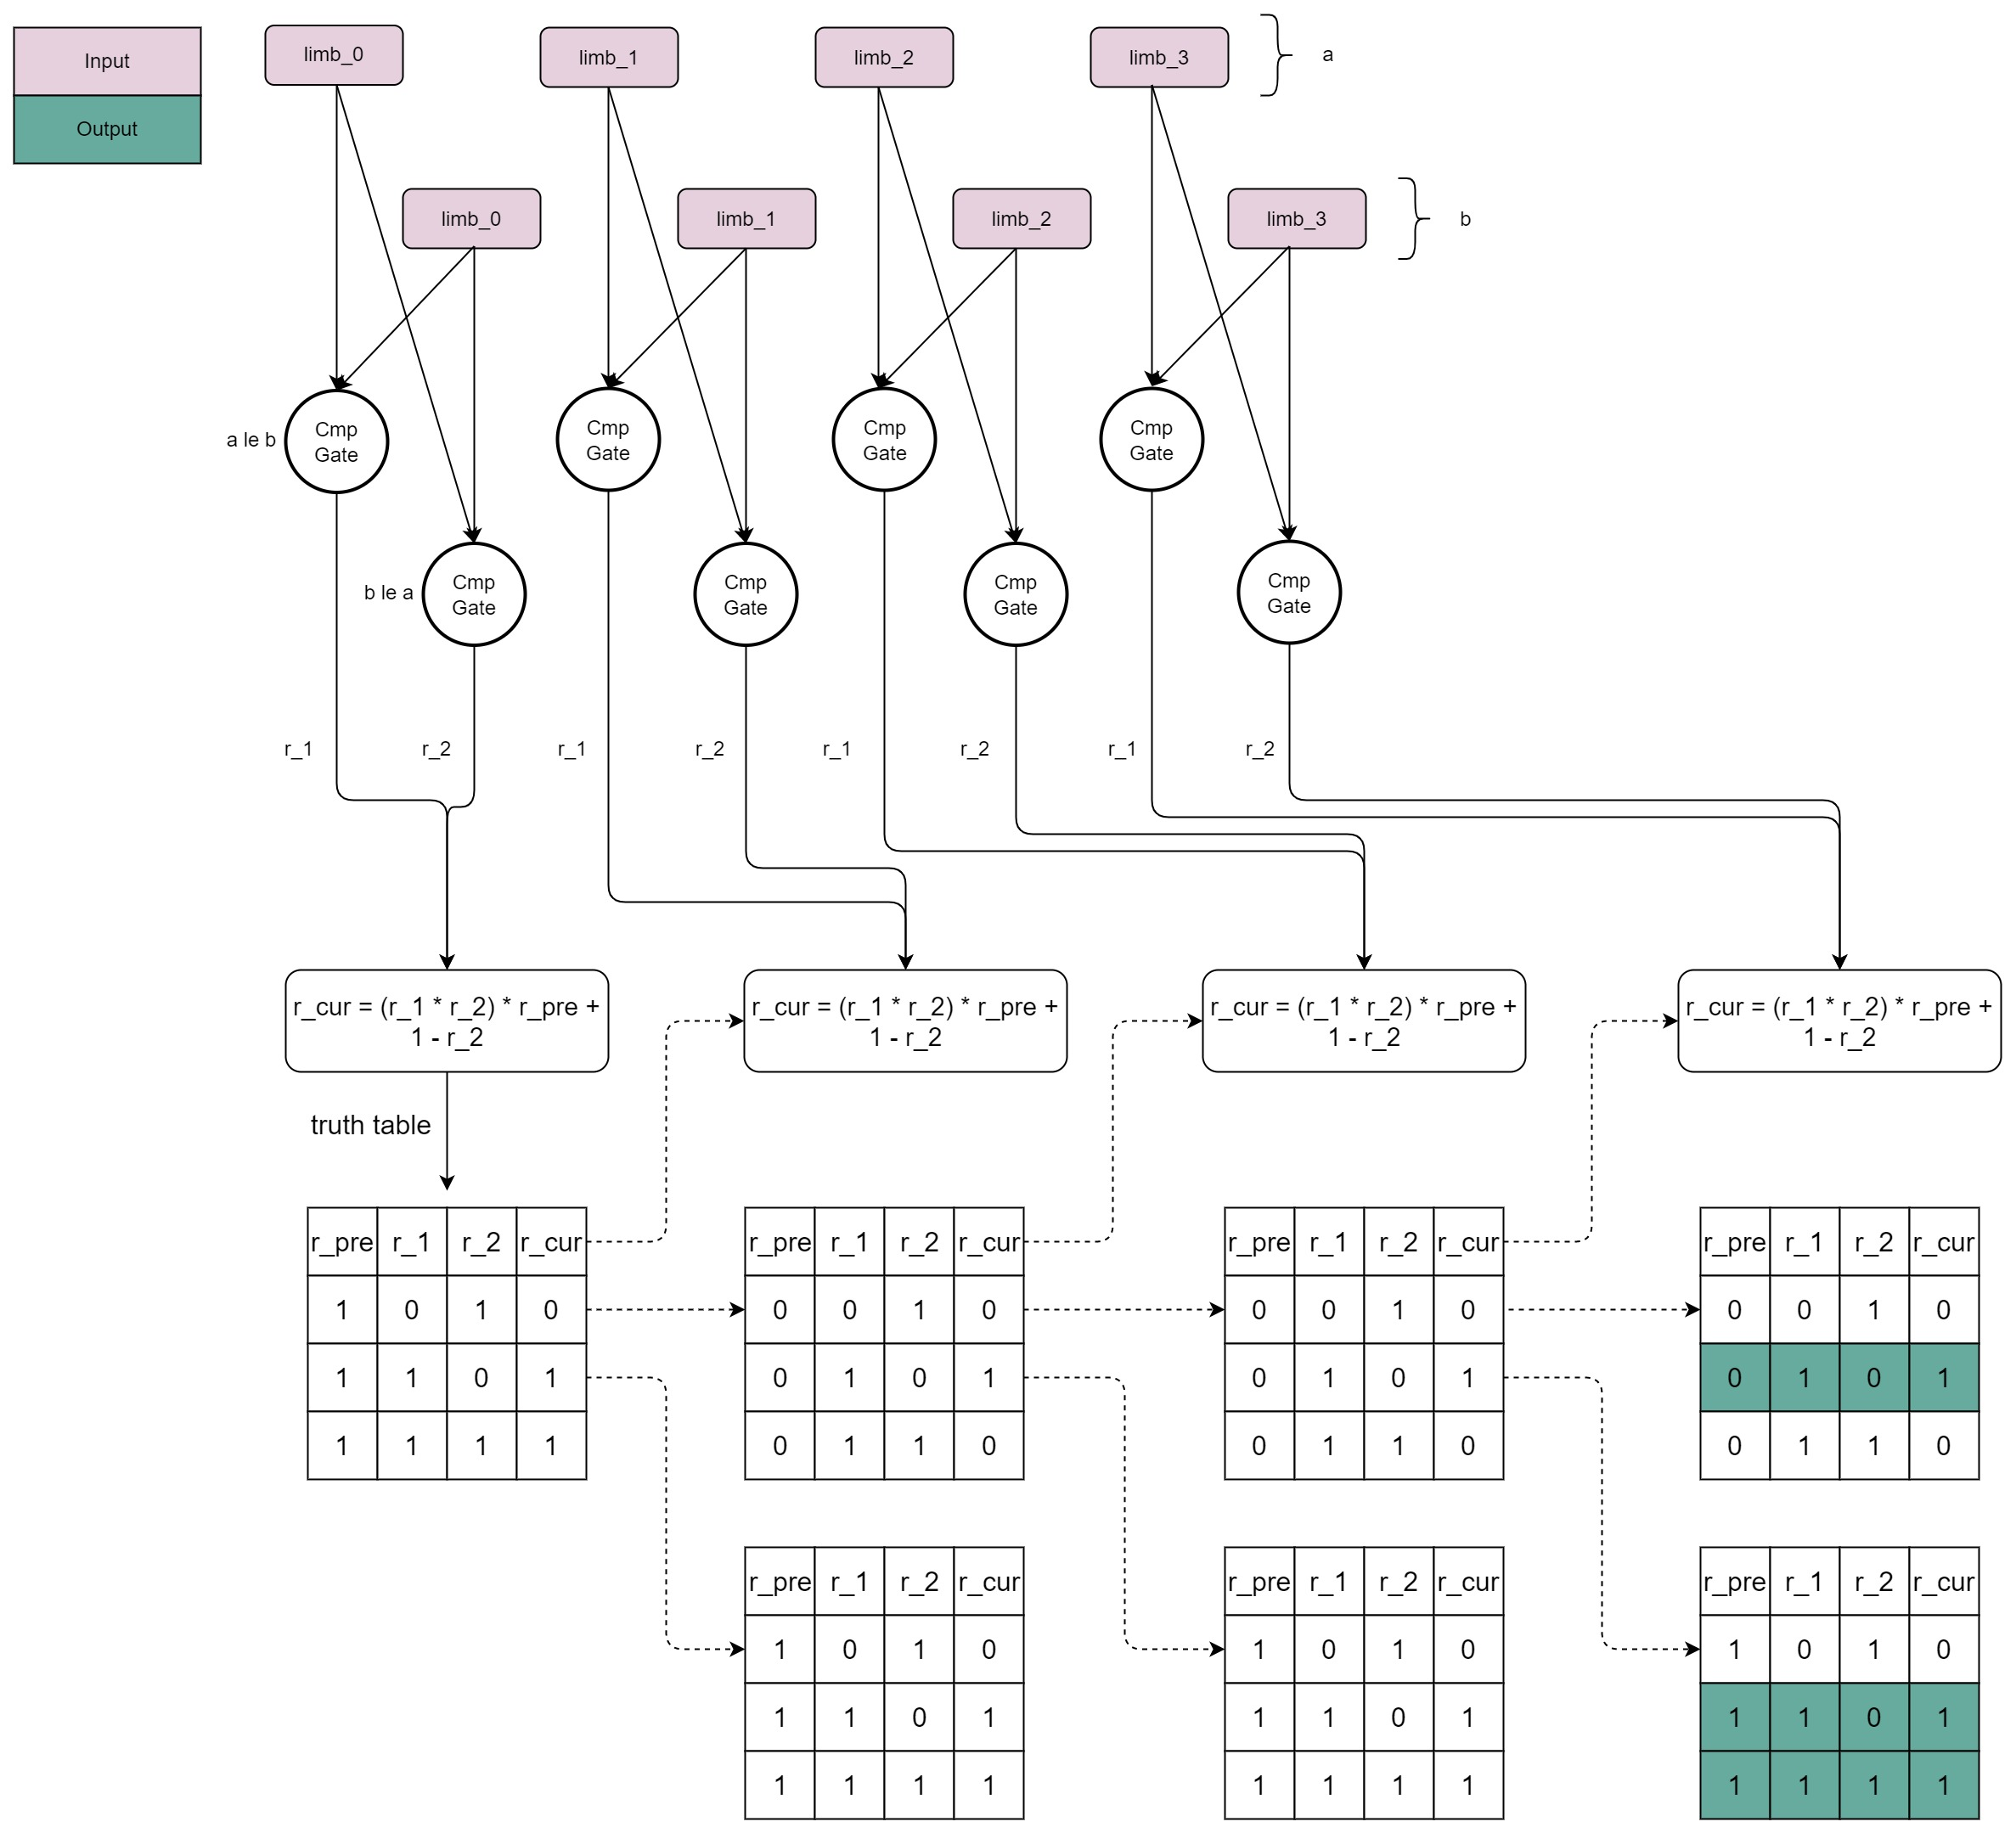
\includegraphics[width=0.8\textwidth]{biguint-cmp-layout.jpg}
    \caption{biguint-cmp layout}
    \label{fig:biguint-cmp-layout}
\end{figure}

\Par{Circuit layout}
See \figref{fig:biguint-cmp-circuit-layout}.
\begin{figure}[!ht]
    \centering
    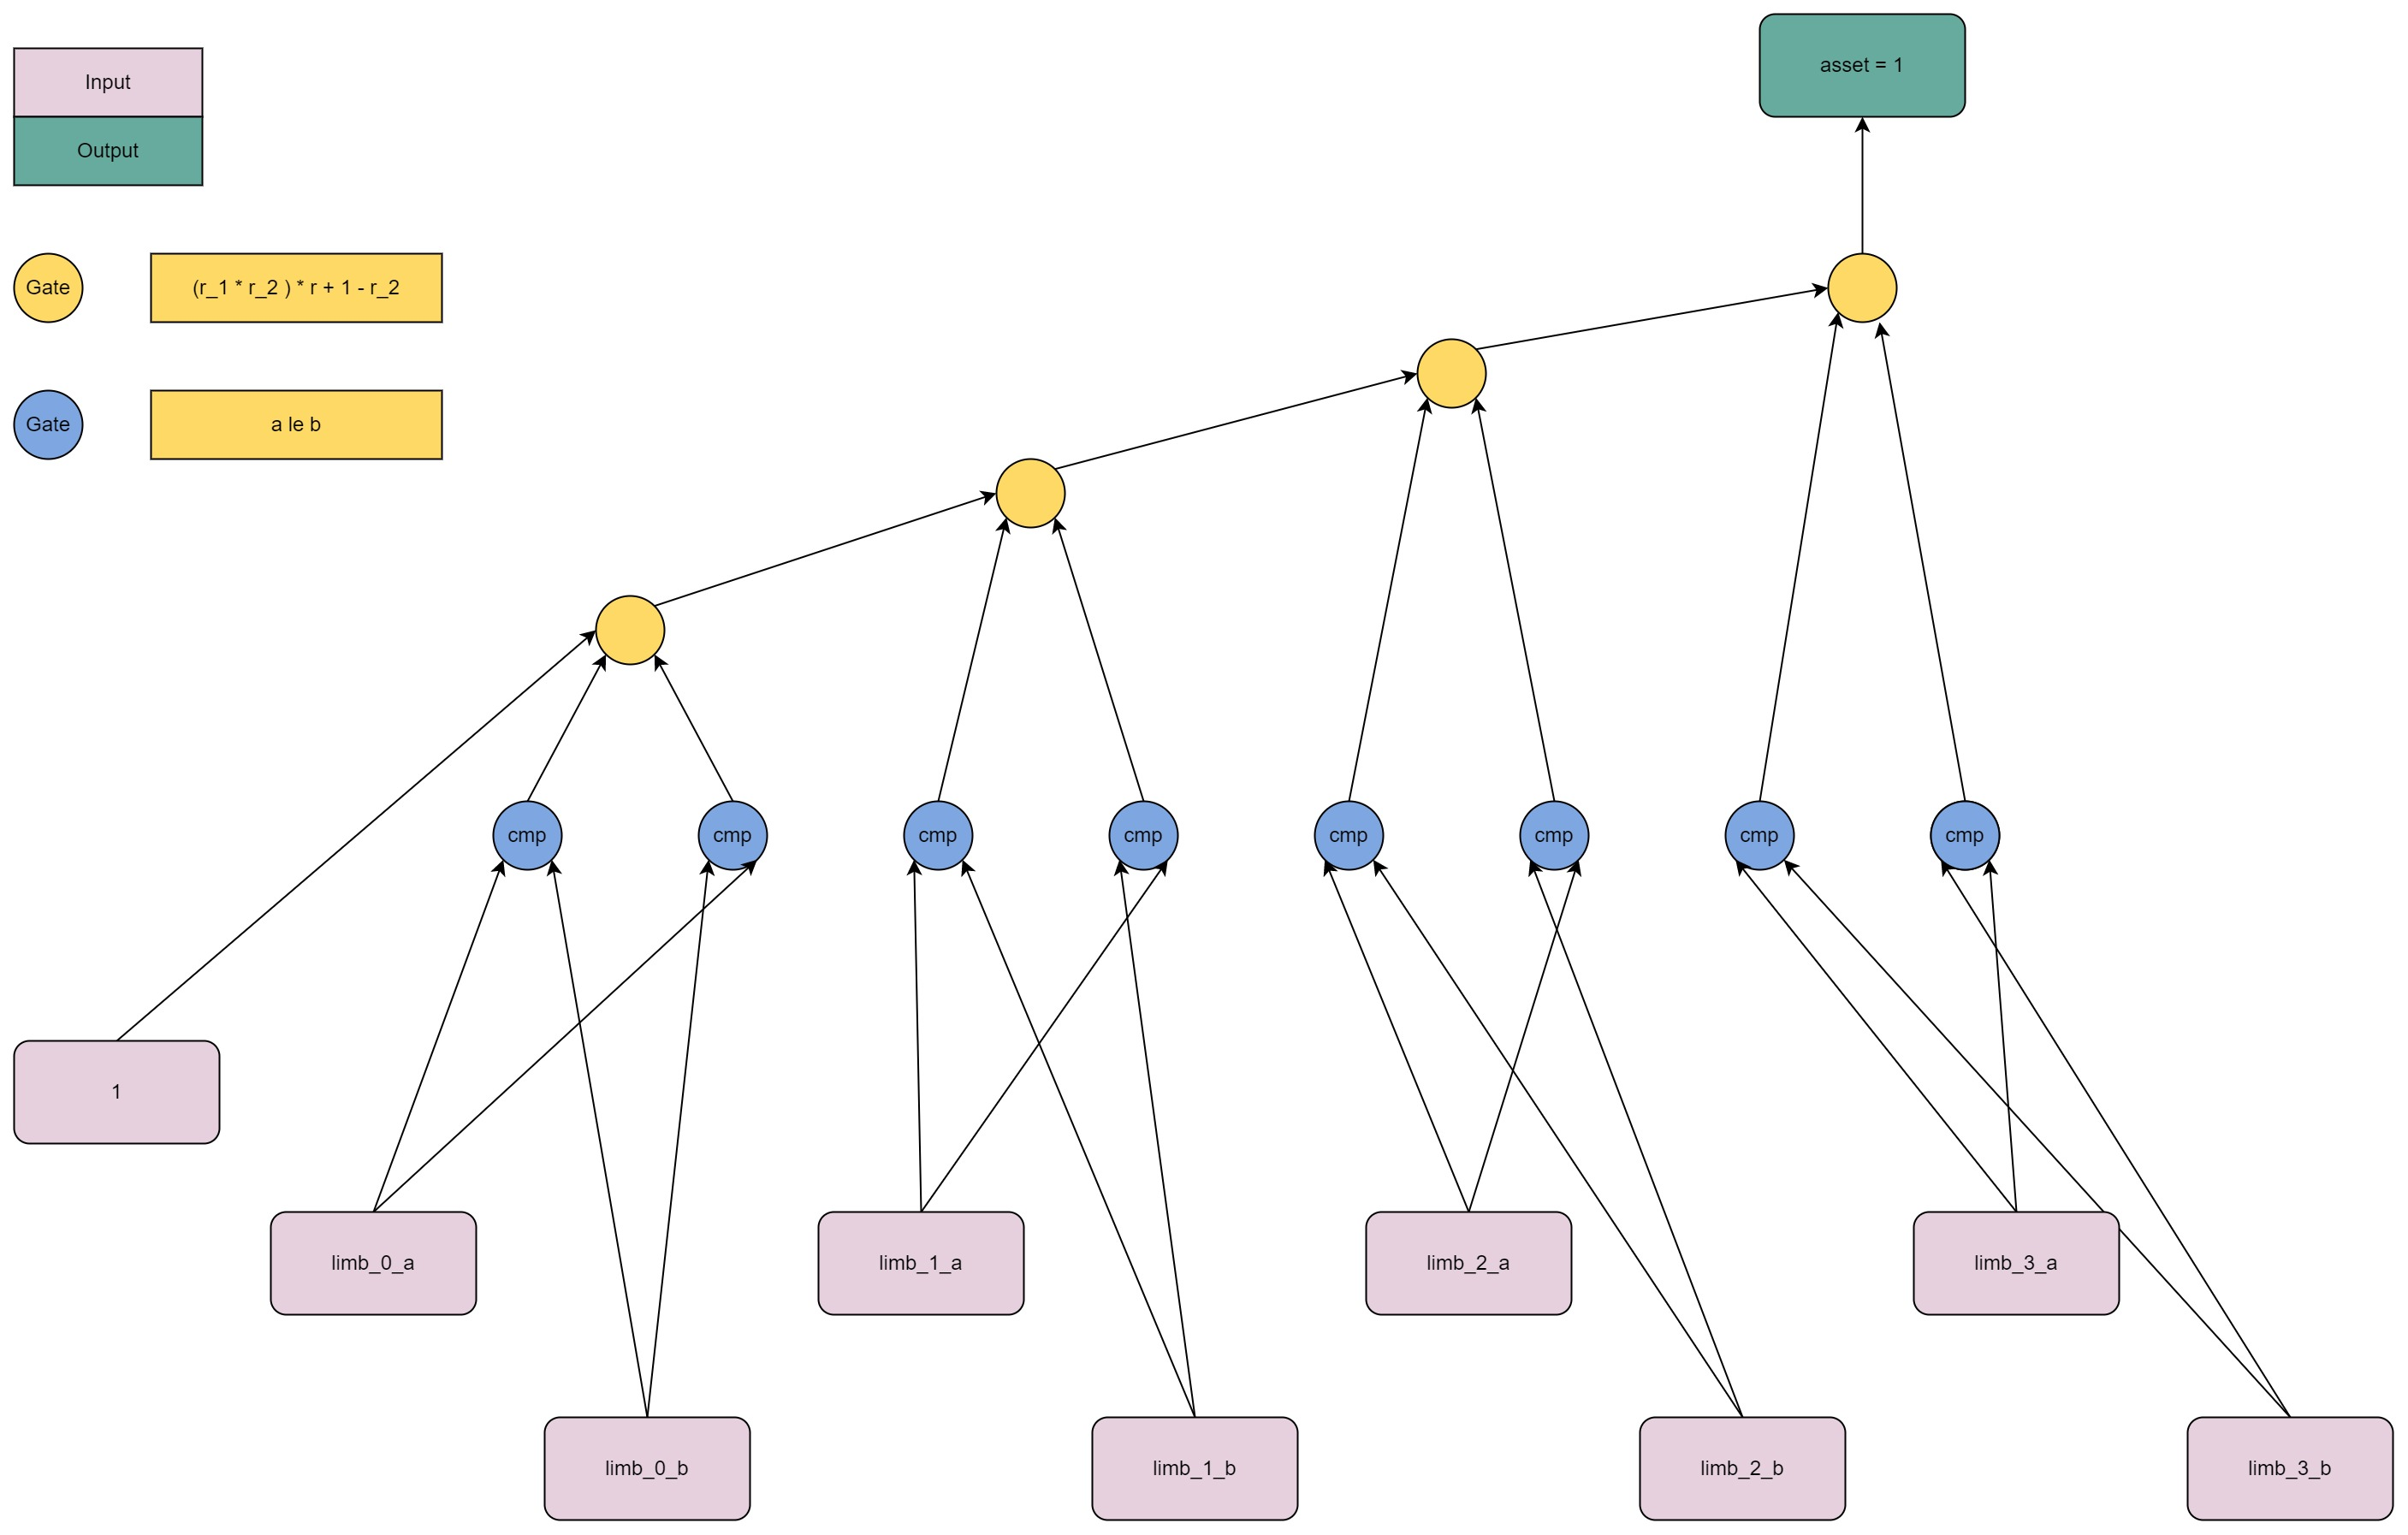
\includegraphics[width=0.8\textwidth]{biguint-cmp-circuit-layout.jpg}
    \caption{biguint-cmp circuit layout}
    \label{fig:biguint-cmp-circuit-layout}
\end{figure}

\Par{Constraints info and costs}
\begin{itemize}
    \item Gate type num: 2 (ComparisionGate, ArithmeticGate)
    \item Gate instance num: $4 \times 2 + 3 = 11$
    \item ComparisionGate num: 8
    \item ArithmeticGate num: 3
    \item copy-constraints: $(4 + 9) \times 4 + 1 = 53$
    \item max-degree: 4
\end{itemize}
